%!TEX root = ../thesis.tex
\newchap{Theoretical framework}\label{sec:TH}
\minitoc
The Standard Model of particle physics (SM) is a quantum field theory that describes all the fundamental forces known beside gravity: the electromagnetic, the strong and the weak force. \\
A quantum field theory (QFT) is a framework that combines quantum mechanics, classical field theory and special relativity, allowing us to describe a particle as the excitation of a quantum field or, more formally, with an irreducible representation of the Poisson group that is characterized by its mass, spin, and additional quantum numbers.
Such theories are characterized by a Lagrangian density $\Lg{}$ that must be Lorentz invariant and must respect locality. \\
In the SM, additional local symmetries (Gauge symmetries) are imposed to describe the interactions between particles and for each symmetry, according to the Noether theorem, a conserved charge arises.

\subsubsection*{Particles of the Standard Model}
Particles are divided into two main categories:
\begin{itemize}
    \item \textbf{Fermions} that have half integer spin:
    \begin{itemize}
        \item obey to the Fermi-Dirac statistics and to the Pauli principle
        \item each fermion has an antiparticle with the same mass but opposite quantum numbers.
    \end{itemize}
    \item \textbf{Bosons} that have integer spin:
    \begin{itemize}
        \item obey the Bose-Einstein statistics
        \item in the SM are the mediators of the interactions.
    \end{itemize}
\end{itemize}

\begin{figure}
    \centering
    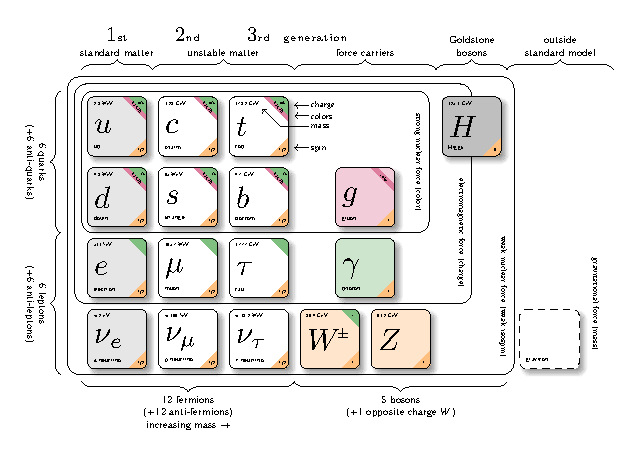
\includegraphics[width=1\linewidth]{fig//chap02-theory/sm-particles.pdf}
    \caption{\cite{BurgardCarstenStandardExample}}
    \label{fig:SMpart}
\end{figure}

\section{The Standard Model of particle physics}

\subsection{Quantum chromodynamics}

\subsection{Electroweak theory}

\subsubsection*{Cabbibo-Kobayashi-Maskawa matrix}

\subsection{The Higgs mechanism}

\section{The $V_{cb}$ element}

\subsection{Measurement with B mesons semileptonic decays}

\subsubsection*{Inclusive measurement}

\subsubsection*{Exclusive measurement}
